\chapter{Disequazioni di secondo grado}
\label{cha:Disequazionisecondogrado}
\section{Disequazioni intere}
Una disequazione di secondo grado\index{Disequazione!secondo grado!intera} è un'espressione del tipo
\begin{equation}
2x^2-x-1\geq 0\label{equ:DisSecondoGrado1}
\end{equation} 
in cui abbiamo un trinomio posto maggiore o uguale di zero. Per risolvere la disequazione  possiamo procedere in questo modo. Trasformiamo  il problema in un altro. Per far ciò  utilizziamo la relazione
\begin{align}
&ax^2+bx+c=a(x-x_{1})(x-x_{2})\label{DisTrinsecGrado0}\\
&x_{1}=\dfrac{-b+\sqrt{b^2-4ac}}{2a}\label{DisTrinsecGrado1}\\
&x_{2}=\dfrac{-b-\sqrt{b^2-4ac}}{2a}\label{DisTrinsecGrado2}
\end{align}
Quindi utilizzando le relazioni\nobs\vrefrange{DisTrinsecGrado0}{DisTrinsecGrado2} possiamo scrivere 
\begin{align}
&2x^2-x-1\\
&x_{1}=\dfrac{1+\sqrt{9}}{4}\notag
&x_{1}=\dfrac{1-\sqrt{9}}{4}\notag\\
&x_{1}=\dfrac{1+3}{4}\notag
&x_{1}=\dfrac{1-3}{4}\notag\\
&x_{1}=\dfrac{4}{4}=1\notag
&x_{1}=-\dfrac{2}{4}=-\dfrac{1}{2}\notag\\
&2x^2-x-1=2(x-1)(x+\dfrac{1}{2})\label{DisTrinsecGradoEs1}
\end{align}
La relazione\nobs\vref{DisTrinsecGradoEs1} trasforma un trinomio di secondo grado nel prodotto di due binomi e un numero. Quindi la disequazione\nobs\vref{equ:DisSecondoGrado1} diventa 
\begin{equation}
2(x-1)(x+\dfrac{1}{2})\geq 0\label{equ:DisSecondogrado1a}
\end{equation} 
Ottengo il grafico\nobs\vref{fig:esempioDisSecGrad1}. Il disegno mostra tre righe una per ogni fattore del prodotto\nobs\vref{equ:DisSecondogrado1a}. Nel particolare il trinomio è positivo per $x\leq-\dfrac{1}{2}$ o $x\geq 1$ negativo per $-\dfrac{1}{2}\leq x\leq 1$

Consideriamo un altro esempio
\begin{equation}
-3x^2+4x-1\geq 0\label{equ:DisSecondoGrado2}
\end{equation} 
anche qui abbiamo un trinomio posto maggiore o uguale di zero. Per risolvere la disequazione  procediamo come prima  Trasformando  il problema in un altro. 
Quindi utilizzando le relazioni\nobs\vrefrange{DisTrinsecGrado0}{DisTrinsecGrado2} possiamo scrivere: 
\begin{align}
&-3x^2+4x-1\\
&x_{1}=\dfrac{-4+\sqrt{4}}{-6}\notag
&x_{1}=\dfrac{-4-\sqrt{4}}{-6}\notag\\
&x_{1}=\dfrac{-4+2}{-6}\notag
&x_{1}=\dfrac{-4-2}{-6}\notag\\
&x_{1}=\dfrac{-2}{-6}=\dfrac{1}{3}\notag
&x_{1}=-\dfrac{-6}{-6}=1\notag\\
&-3x^2+4x-1=-3(x-1)(x-\dfrac{1}{3})\label{DisTrinsecGradoEs2}
\end{align}
Anche questa volta relazione\nobs\vref{DisTrinsecGradoEs2} trasforma il trinomio di secondo grado nel prodotto di due binomi e un numero. Quindi la disequazione\nobs\vref{equ:DisSecondoGrado2} diventa 
\begin{equation}
-3(x-1)(x-\dfrac{1}{3})\geq 0\label{equ:DisSecondogrado2a}
\end{equation} 
Ottengo il grafico\nobs\vref{fig:esempioDisSecGrad2}. Il disegno mostra tre righe una per ogni fattore del prodotto\nobs\vref{equ:DisSecondogrado2a}. Nel particolare il trinomio è negativo per $x\leq\dfrac{1}{3}$ o $x\geq 1$, positivo per $-\dfrac{1}{3}\leq x\leq 1$
\begin{figure}
	\centering
		\begin{subfigure}[b]{.4\linewidth}
			\centering
			\includestandalone[width=\textwidth]{quarto/DisSecGrado/DisSecGradoesempio1}
			\caption{Esempio 1}
			\label{fig:esempioDisSecGrad1}
		\end{subfigure}%
	\centering
	\begin{subfigure}[b]{.4\linewidth}
			\centering
			\includestandalone[width=\textwidth]{quarto/DisSecGrado/DisSecGradoesempio2}
			\caption{Esempio 2}
			\label{fig:esempioDisSecGrad2}
	\end{subfigure}%
\caption{$\Delta>0$}
\label{fig:DeltaMagZeroEsempio1}
\end{figure}

La figura\nobs\vref{fig:DeltaMagZeroEsempio1} permette di confrontare i due grafici. Questi sono praticamente identici. \'{E} la terza riga, continua nel primo esempio, tratteggiata nel secondo, che fa la differenza. Guardando i due grafici, vediamo che all'esterno dell'intervallo formato dalle due soluzioni, il grafico ha lo stesso segno del coefficiente $a$. Mentre nello spazio compreso fra le due soluzioni, il segno è opposto a quello di $a$. Otteniamo due grafici come\nobs\vrefrange{graf:dis2GDeltaMagZa2x}{graf:dis2GDeltaMagZb2x}. Questo è riassunto graficamente dalla prima riga della tabella\nobs\vref{tab:segnodisequazioni2grado}
\begin{figure}
	\begin{subfigure}[b]{.5\linewidth}
		\centering
\includestandalone[width=\textwidth]{quarto/DisSecGrado/DeltaMaggioreDiZeroAmaggioreDizero}
		\caption{$\Delta>0$ $a>0$}\label{graf:dis2GDeltaMagZa2x}
	\end{subfigure}%
	\begin{subfigure}[b]{.5\linewidth}
		\centering
	\includestandalone[width=\textwidth]{quarto/DisSecGrado/DeltaMaggioreDiZeroAminoreDizero}
		\caption{$\Delta>0$ $a<0$}\label{graf:dis2GDeltaMagZb2x}
	\end{subfigure}
	\begin{subfigure}[b]{.5\linewidth}
		\centering
		\includestandalone[width=\textwidth]{quarto/DisSecGrado/DeltaUgualeaZeroAmaggioreDizero}
		\caption{$\Delta=0$ $a>0$}\label{graf:dis2GDeltaUguaZa2x}
			\end{subfigure}%
	\begin{subfigure}[b]{.5\linewidth}
		\centering
		\includestandalone[width=\textwidth]{quarto/DisSecGrado/DeltaUgualeaZeroAminoreDizero}
		\caption{$\Delta=0$ $a<0$}\label{graf:dis2GDeltaUguaZb2x}
	\end{subfigure}
\begin{subfigure}[b]{.5\linewidth}
	\centering
		\includestandalone[width=\textwidth]{quarto/DisSecGrado/DeltaMinoreZeroAmaggioreDizero}
	\caption{$\Delta<0$ $a>0$}\label{graf:dis2GDeltaMinorZa2x}
\end{subfigure}%
\begin{subfigure}[b]{.5\linewidth}
	\centering
\includestandalone[width=\textwidth]{quarto/DisSecGrado/DeltaMinoreZeroAminoreDizero}
	\caption{$\Delta<0$ $a<0$}\label{graf:dis2GDeltaMinorZb2x}
\end{subfigure}
	\caption{Grafici disequazione di secondo grado}
\end{figure}
\begin{table}
	\begin{tabular}{@{}m{0.8cm}m{7.8cm}m{7.8cm}}
		\toprule
		& \centering $a>0$ & \centering$a<0$ \tabularnewline
\centering$\Delta>0$ &\tabincludestandalone[width=7.5cm]{quarto/DisSecGrado/DeltaMaggioreDiZeroAmaggioreDizero}  & 	\tabincludestandalone[width=7.5cm]{quarto/DisSecGrado/DeltaMaggioreDiZeroAminoreDizero} \\[0.5cm] 
		\centering$\Delta=0$ & 	\tabincludestandalone[width=7.5cm]{quarto/DisSecGrado/DeltaUgualeaZeroAmaggioreDizero} &  \tabincludestandalone[width=7.5cm]{quarto/DisSecGrado/DeltaUgualeaZeroAminoreDizero}\\[0.5cm] 
		\centering$\Delta<0$ & \tabincludestandalone[width=7.5cm]{quarto/DisSecGrado/DeltaMinoreZeroAmaggioreDizero} & \tabincludestandalone[width=7.5cm]{quarto/DisSecGrado/DeltaMinoreZeroAminoreDizero}\\[0.5cm] 
		\bottomrule
	\end{tabular}
	\caption{Segno disequazioni secondo grado}
\end{table}
\begin{table}
	\centering
	\begin{tikzpicture}
	\tkzTabInit[color,lgt=5,espcl=3]%
	{$x$ / .8,$\Delta>0$\\ Il segno di\\ $ax^2+bx+c$ /2}%
	{$-\infty$,$x_1$,$x_2$,$+\infty$}%
	\tkzTabLine{ , \genfrac{}{}{0pt}{0}{\text{segno di}}{a}, z
		, \genfrac{}{}{0pt}{0}{\text{segno}}{\text{opposto di}\ a}, z
		, \genfrac{}{}{0pt}{0}{\text{segno di}}{a}, }
	\end{tikzpicture}\\
	\begin{tikzpicture}
	\tkzTabInit[color,lgt=5,espcl=3]%
	{$x$ / .8, $\Delta=0$\\ Il segno di\\ $ax^2+bx+c$ / 2}%
	{$-\infty$,$x_1$,$+\infty$}%
	\tkzTabLine{ , \genfrac{}{}{0pt}{0}{\text{segno di}}{ a} , z
		, \genfrac{}{}{0pt}{0}{\text{segno di}}{a}, }
	\end{tikzpicture}\\
	\begin{tikzpicture}
	\tkzTabInit[color,lgt=5,espcl=5]%
	{$x$/.8,$\Delta<0$\\ Il segno di\\ $ax^2+bx+c$/2}%
	{$-\infty$,$+\infty$}%
	\tkzTabLine{ , \genfrac{}{}{0pt}{0}{\text{segno di}}{ a}, }
	\end{tikzpicture}
	\caption{Segno disequazione di secondo grado}
	\label{tab:segnodisequazioni2grado}
\end{table}

Consideriamo una disequazione del tipo
\begin{equation}
2x^2-4x+2\geq 0\label{equ:DisSecondoGrado3}
\end{equation} 
come negli esempi precedenti abbiamo un trinomio di secondo grado  posto maggiore o uguale di zero. Anche qui trasformiamo  il problema in un altro. Per far ciò  utilizziamo le relazioni\nobs\vrefrange{DisTrinsecGrado0}{DisTrinsecGrado2}.
Possiamo scrivere:
\begin{align}
&2x^2-4x+2\\
&x_{1}=\dfrac{4+\sqrt{0}}{4}\notag
&x_{1}=\dfrac{4-\sqrt{0}}{4}\notag\\
&x_{1}=\dfrac{4}{4}=1\notag
&x_{1}=\dfrac{4}{4}=1\notag\\
&2x^2-4x+2=2(x-1)(x-1)=2(x-1)^2\label{DisTrinsecGradoEs3}
\end{align}
La relazione\nobs\vref{DisTrinsecGradoEs1} trasforma un trinomio di secondo grado nel prodotto di un binomio al quadrato e un numero. Quindi la disequazione\nobs\vref{equ:DisSecondoGrado3} diventa 
\begin{equation}
2(x-1)^2\geq 0\label{equ:DisSecondogrado3a}
\end{equation} 
Ottengo il grafico\nobs\vref{fig:esempioDisSecGrad3}. Il disegno mostra tre righe una per ogni fattore del prodotto\nobs\vref{equ:DisSecondogrado3a}. Nel particolare il trinomio è positivo per $x1$ e $x>1$, vale zero  per $x=1$
\begin{figure}
	\centering
	\begin{subfigure}[b]{.4\linewidth}
		\centering
		\includestandalone[width=\textwidth]{quarto/DisSecGrado/DisSecGradoesempio3}
		\caption{Esempio 3}
		\label{fig:esempioDisSecGrad3}
	\end{subfigure}%
	\centering
	\begin{subfigure}[b]{.4\linewidth}
		\centering
		\includestandalone[width=\textwidth]{quarto/DisSecGrado/DisSecGradoesempio4}
		\caption{Esempio 4}
		\label{fig:esempioDisSecGrad4}
	\end{subfigure}%
	\caption{$\Delta=0$}
	\label{fig:DeltaUguZeroEsempio2}
\end{figure}

Continuiamo con gli esempi
\begin{equation}
-3x^2+12x-12\geq 0\label{equ:DisSecondoGrado4}
\end{equation} 
come in precedenza abbiamo un trinomio di secondo grado  posto maggiore o uguale di zero.  Utilizziamo anche qui le relazioni\nobs\vrefrange{DisTrinsecGrado0}{DisTrinsecGrado2}.
Possiamo scrivere:
\begin{align}
&-3x^2+12x-12\\
&x_{1}=\dfrac{-12+\sqrt{0}}{-6}\notag
&x_{1}=\dfrac{-12-\sqrt{0}}{-6}\notag\\
&x_{1}=\dfrac{-12}{-6}=2\notag
&x_{1}=\dfrac{-12}{-6}=2\notag\\
&-3x^2+12x-12=-3(x-2)(x-2)=-3(x-2)^2\label{DisTrinsecGradoEs4}
\end{align}
La relazione\nobs\vref{DisTrinsecGradoEs1} trasforma un trinomio di secondo grado nel prodotto di un binomio al quadrato e un numero. Quindi la disequazione\nobs\vref{equ:DisSecondoGrado4} diventa 
\begin{equation}
-3(x-2)^2\geq 0\label{equ:DisSecondogrado4a}
\end{equation} 
Ottengo il grafico\nobs\vref{fig:esempioDisSecGrad4}. Il disegno mostra tre righe una per ogni fattore del prodotto\nobs\vref{equ:DisSecondogrado4a}. Nel particolare il trinomio è negativo per $x<2$ e $x>2$, vale zero  per $x=2$

Confrontiamo i due grafici tramite la figura\nobs\vref{fig:DeltaUguZeroEsempio2}. Anche  la terza  riga, continua nel primo esempio, tratteggiata nel secondo, fa la differenza. Guardando i due grafici, vediamo che il grafico ha lo stesso segno del coefficiente $a$ tranne per $x=x_1$ in cui vale zero.  come\nobs\vrefrange{graf:dis2GDeltaUguaZa2x}{graf:dis2GDeltaUguaZb2x}. Questo è riassunto graficamente dalla seconda riga della tabella\nobs\vref{tab:segnodisequazioni2grado}

Nella prima coppia di esempi avevamo due soluzioni distinte, nella seconda le soluzioni erano coincidenti. Resta da considerare quando le soluzioni non esistono.

In questo caso il discriminate dell'equazione è un numero minore di zero. Si può dimostrare con qualche calcolo in più che i grafici sono come quelli delle figure\nobs\vrefrange{graf:dis2GDeltaMinorZa2x}{graf:dis2GDeltaMinorZb2x}. In questo caso il grafico ha sempre lo stesso segno di $a$  nella terza riga della tabella\nobs\vref{tab:segnodisequazioni2grado}
\begin{table}
	\centering
	 \begin{tabular}{@{}cc>{\centering}m{6.5cm}>{\centering}m{6.5cm}}
	 	&  & $a>0$ &  $a<0$ \tabularnewline[0.5cm] 
	 	&  & 	\tabincludestandalone[width=6.5cm]{quarto/DisSecGrado/DeltaMaggioreDiZeroAmaggioreDizero}  & 	\tabincludestandalone[width=6.5cm]{quarto/DisSecGrado/DeltaMaggioreDiZeroAminoreDizero} \tabularnewline[0.5cm] 
	 	\multirow{4}{1cm}{$\Delta>0$}	& $ax^2+bx+c\geq 0$ & $x\leq x_1$ e $x\geq x_2$  & $x_1\leq x \leq x_2$ \tabularnewline  
	 	& $ax^2+bx+c > 0$ &$x< x_1$ e $x>x_2$  & $x_1< x < x_2$ \tabularnewline
	 	& $ax^2+bx+c\leq 0$ & $x_1\leq x \leq x_2$ & $x\leq x_1$ e $x\geq x_2$ \tabularnewline  
	 	& $ax^2+bx+c< 0$ & $x_1< x < x_2$ & $x< x_1$ e $x>x_2$ \tabularnewline
	 	&  & 	\tabincludestandalone[width=6.5cm]{quarto/DisSecGrado/DeltaUgualeaZeroAmaggioreDizero} &  \tabincludestandalone[width=6.5cm]{quarto/DisSecGrado/DeltaUgualeaZeroAminoreDizero}\tabularnewline[0.5cm] 
	 	\multirow{4}{1cm}{$\Delta=0$}	& $ax^2+bx+c\geq 0$ & Sempre & $x=x_1$ \tabularnewline  
	 	& $ax^2+bx+c > 0$ & Sempre $x\neq x_1$ & Mai \tabularnewline
	 	& $ax^2+bx+c\leq 0$ & $x=x_1 $  & Sempre \tabularnewline  
	 	& $ax^2+bx+c< 0$ & Mai & Sempre $x\neq x_1$ \tabularnewline  
	 	&  & 	\tabincludestandalone[width=6.5cm]{quarto/DisSecGrado/DeltaMinoreZeroAmaggioreDizero} & \tabincludestandalone[width=6.5cm]{quarto/DisSecGrado/DeltaMinoreZeroAminoreDizero}\tabularnewline[0.5cm] 
	 	\multirow{4}{1cm}{$\Delta<0$}	& $ax^2+bx+c\geq 0$ & Sempre. Uguale a zero mai & Mai \tabularnewline  
	 	& $ax^2+bx+c > 0$ & Sempre & Mai \tabularnewline
	 	& $ax^2+bx+c\leq 0$ & Mai & Sempre. Uguale a zero mai \tabularnewline  
	 	& $ax^2+bx+c< 0$ & Mai & Sempre \tabularnewline  
	 \end{tabular} 
	\caption{Soluzioni disequazioni secondo grado}
	\label{tab:SoluzioniDisequazioniSecondoGrado}
\end{table}
   
\altapriorita{aggiungere disequazioni frazionarie di secondo grado}
% % % % % % % % % % % % % % % % % % % % % % % % % % % % %
%\section{Metodo grafico}
%\label{sec:MetodoGrafico}
%\begin{figure}
%	
%		\begin{subfigure}[b]{.5\linewidth}
%		\centering
%		\begin{tikzpicture}[line cap=round,line join=round,>=triangle 45,x=1.0cm,y=1.0cm]
%		\draw[->,color=black] (-3,0) -- (3,0);
%		%\foreach \x in {-2.5,-2,-1.5,-1,-0.5,0.5,1,1.5,2,2.5,3}
%		%\draw[shift={(\x,0)},color=black] (0pt,-2pt);
%		\clip(-3,-2.28) rectangle (3,1);
%		\draw [samples=50,rotate around={0:(0,-2.13)},xshift=0cm,yshift=-2.13cm] %plot (\x,\x^2/2/0.2599999999999998);
%		plot(\x,{(\x)^2-0.1}); 
%		%\draw [samples=50,rotate around={0:(0,-2.13)},xshift=0cm,yshift=-2.13cm] plot (\x,(\x)^2/2/0.2599999999999998);
%		\draw (-3,0.37) node[anchor=north west] {$+++++$};
%		\draw (-1.17,0.05) node[anchor=north west] {$x_1$};
%		\draw (1.11,0.05) node[anchor=north west] {$x_2$};
%		\draw (1.17,0.37) node[anchor=north west] {$++++++$};
%		\draw (-0.7,-0.06) node[anchor=north west] {$-----$};
%		\end{tikzpicture}
%		\caption{$\Delta>0$ $a>0$}\label{graf:dis2GDeltaMagZGa1}
%	\end{subfigure}%
%	\begin{subfigure}[b]{.5\linewidth}
%		\centering
%			\begin{tikzpicture}[line cap=round,line join=round,>=triangle 45,x=1.0cm,y=1.0cm]
%			\draw[->,color=black] (-3,0) -- (3,0);
%			%\foreach \x in {-3,-2.5,-2,-1.5,-1,-0.5,0.5,1,1.5,2,2.5}
%			%\draw[shift={(\x,0)},color=black] (0pt,-2pt);
%			\clip(-3,-1) rectangle (3,2.26);
%			\draw [samples=50,rotate around={-180:(0,2.13)},xshift=0cm,yshift=2.13cm] 
%			%plot (\x,\x^2/2/0.2599999999999998);
%			plot(\x,{(-\x)^2-0.1}); 
%			\draw (-0.8,0.37) node[anchor=north west] {$+++++$};
%			\draw (-1.17,0.04) node[anchor=north west] {$x_1$};
%			\draw (1.11,0.06) node[anchor=north west] {$x_2$};
%			\draw (-3,-0.37) node[anchor=north west] {$-----$};
%			\draw (1.39,-0.37) node[anchor=north west] {$-----$};
%			\end{tikzpicture}
%		\caption{$\Delta>0$ $a<0$}\label{graf:dis2GDeltaMagZGb1}
%	\end{subfigure}
%		\begin{subfigure}[b]{.5\linewidth}
%			\centering
%			\begin{tikzpicture}[line cap=round,line join=round,>=triangle 45,x=1.0cm,y=1.0cm]
%			\draw[->,color=black] (-3,0) -- (3,0);
%			%\foreach \x in {-3,-2.5,-2,-1.5,-1,-0.5,0.5,1,1.5,2,2.5}
%			%\draw[shift={(\x,0)},color=black] (0pt,-2pt);
%			\clip(-3,-0.3) rectangle (3,0.5);
%			\draw (-1,0.5)-- (-1,0);
%			\draw (1,0.5)-- (1,0);
%			\draw [line width=1.2pt,dash pattern=on 5pt off 5pt] (-1,0.5) -- (1,0.5);
%			\draw (1,0.5)-- (3,0.5);
%			\draw (-1,0.5)-- (-3,0.5);
%			\draw (-1.02,0.02) node[anchor=north west] {$x_1$};
%			\draw (0.98,0.02) node[anchor=north west] {$x_2$};
%			\end{tikzpicture}
%			\caption{$\Delta>0$ $a>0$}\label{graf:dis2GDeltaMagZGa2}
%		\end{subfigure}%
%		\begin{subfigure}[b]{.5\linewidth}
%			\centering
%				\begin{tikzpicture}[line cap=round,line join=round,>=triangle 45,x=1.0cm,y=1.0cm]
%				\draw[->,color=black] (-3,0) -- (3,0);
%				%\foreach \x in {-3,-2.5,-2,-1.5,-1,-0.5,0.5,1,1.5,2,2.5}
%				%\draw[shift={(\x,0)},color=black] (0pt,-2pt);
%				\clip(-3,-0.3) rectangle (3,0.5);
%				\draw (-1,0.5)-- (-1,0);
%				\draw (1,0.5)-- (1,0);
%				\draw (-1,0.5)-- (1,0.5);
%				\draw [dash pattern=on 5pt off 5pt] (1,0.5)-- (3.0,0.5);
%				\draw [dash pattern=on 5pt off 5pt] (-1,0.5)-- (-3.0,0.5);
%				\draw (-1.02,0.02) node[anchor=north west] {$x_1$};
%				\draw (0.98,0.02) node[anchor=north west] {$x_2$};
%				\end{tikzpicture}
%			\caption{$\Delta>0$ $a<0$}\label{graf:dis2GDeltaMagZGb2}
%		\end{subfigure}
%	\caption{$\Delta>0$}%
%	\label{fig:deltamz}
%\end{figure}
%
%\begin{figure}
%	\begin{subfigure}[b]{.5\linewidth}
%		\centering
%			\begin{tikzpicture}[line cap=round,line join=round,>=triangle 45,x=1.0cm,y=1.0cm]
%			\draw[->,color=black] (-3,0) -- (2.98,0);
%			%\foreach \x in {-3,-2.5,-2,-1.5,-1,-0.5,0.5,1,1.5,2,2.5}
%			%\draw[shift={(\x,0)},color=black] (0pt,-2pt);
%			\clip(-3,-0.29) rectangle (2.98,2);
%			\draw [samples=50,rotate around={0:(0,0)},xshift=0cm,yshift=0cm]
%			%plot (\x,\x^2/2/1.0);
%			plot(\x,{(\x)^2}); 
%			\draw (0,0.02) node[anchor=north west] {$x_1$};
%			\draw (-3,0.37) node[anchor=north west] {$+++++++++++++++++++++$};
%			\end{tikzpicture}
%		\caption{$\Delta=0$ $a>0$}\label{graf:dis2GDeltaUguaZGa1}
%	\end{subfigure}%
%	\qquad
%	\begin{subfigure}[b]{.5\linewidth}
%		\centering
%		\begin{tikzpicture}[line cap=round,line join=round,>=triangle 45,x=1.0cm,y=1.0cm]
%		\draw[->,color=black] (-3,0) -- (2.98,0);
%		%\foreach \x in {-3,-2.5,-2,-1.5,-1,-0.5,0.5,1,1.5,2,2.5}
%		%\draw[shift={(\x,0)},color=black] (0pt,-2pt);
%		\clip(-3,-2) rectangle (2.98,0.29);
%		\draw [samples=50,rotate around={-180:(0,0)},xshift=0cm,yshift=0cm] 
%		%plot (\x,\x^2/2/1.0);
%		plot(\x,{(-\x)^2}); 
%		\draw (0,0.02) node[anchor=north west] {$x_1$};
%		\draw (-3,0.37) node[anchor=north west] {$---------------------$};
%		\end{tikzpicture}
%		\caption{$\Delta=0$ $a<0$}\label{graf:dis2GDeltaDeltaUguaZGb1}
%	\end{subfigure}
%		\begin{subfigure}[b]{.5\linewidth}
%			\centering
%		\begin{tikzpicture}[line cap=round,line join=round,>=triangle 45,x=1.0cm,y=1.0cm]
%		\draw[->,color=black] (-3,0) -- (3,0);
%		%\foreach \x in {-2.5,-2,-1.5,-1,-0.5,0.5,1,1.5,2,2.5,3}
%		%\draw[shift={(\x,0)},color=black] (0pt,-2pt);
%		\clip(-3,-0.3) rectangle (3,0.5);
%		\draw (0,0.5)-- (0,0);
%		\draw [domain=-3:3] plot(\x,{(--0.56-0*\x)/1.12});
%		\draw (-0.03,0.02) node[anchor=north west] {$x_1$};
%		\end{tikzpicture}
%			\caption{$\Delta=0$ $a>0$}\label{graf:dis2GDeltaUguaZGa2}
%		\end{subfigure}%
%		\qquad
%		\begin{subfigure}[b]{.5\linewidth}
%			\centering
%			\begin{tikzpicture}[line cap=round,line join=round,>=triangle 45,x=1.0cm,y=1.0cm]
%			\draw[->,color=black] (-3,0) -- (3,0);
%			\foreach \x in {-2.5,-2,-1.5,-1,-0.5,0.5,1,1.5,2,2.5,3}
%			\draw[shift={(\x,0)},color=black] (0pt,-2pt);
%			\clip(-3,-0.3) rectangle (3,0.5);
%			\draw (0,0.5)-- (0,0);
%			%\draw [domain=-3:3] plot(\x,{(--0.56-0*\x)/1.12});
%			%\draw [dash pattern=on 5pt off 5pt,domain=-3:3] plot(\x,{(--1.18-0*\x)/1.18});
%			\draw [dash pattern=on 5pt off 5pt,domain=-3:3] plot(\x,{(--0.56-0*\x)/1.12});
%			\draw (-0.03,0.02) node[anchor=north west] {$x_1$};
%			\end{tikzpicture}
%			\caption{$\Delta=0$ $a<0$}\label{graf:dis2GDeltaUguaZGb2}
%		\end{subfigure}
%		\caption{$\Delta=0$}%
%		\label{fig:deltaugz}
%\end{figure}
%
%
%\begin{figure}
%	\begin{subfigure}[b]{.5\linewidth}
%		\centering
%		\begin{tikzpicture}[line cap=round,line join=round,>=triangle 45,x=1.0cm,y=1.0cm]
%		\draw[->,color=black] (-3,0) -- (3,0);
%		%\foreach \x in {-3,-2.5,-2,-1.5,-1,-0.5,0.5,1,1.5,2,2.5}
%		%\draw[shift={(\x,0)},color=black] (0pt,-2pt);
%		\clip(-3,-0.3) rectangle (3,2);
%		\draw [samples=50,rotate around={0:(0,0.15)},xshift=0cm,yshift=0.15cm] 
%		plot(\x,{(\x)^2+.2}); 
%		%plot (\x,\x^2/2/0.3);
%		\draw (-3,-0.01) node[anchor=north west] {$+++++++++++++++++++++$};
%		\end{tikzpicture}
%		\caption{$\Delta<0$ $a>0$}\label{graf:dis2GDeltaMinorZGa1}
%	\end{subfigure}%
%	\qquad
%	\begin{subfigure}[b]{.5\linewidth}
%		\centering
%		\begin{tikzpicture}[line cap=round,line join=round,>=triangle 45,x=1.0cm,y=1.0cm]
%		\draw[->,color=black] (-3,0) -- (3,0);
%		%\foreach \x in {-3,-2.5,-2,-1.5,-1,-0.5,0.5,1,1.5,2,2.5}
%		%\draw[shift={(\x,0)},color=black] (0pt,-2pt);
%		\clip(-3,-2) rectangle (3,0.3);
%		\draw [samples=50,rotate around={-180:(0,-0.15)},xshift=0cm,yshift=-0.15cm] 
%		%plot (\x,\x^2/2/0.3);
%		plot(\x,{(-\x)^2+.2}); 
%		\draw (-3,0.37) node[anchor=north west] {$---------------------$};
%		\end{tikzpicture}
%		\caption{$\Delta<0$ $a<0$}\label{graf:dis2GDeltaMinorZGb1}
%	\end{subfigure}
%	\begin{subfigure}[b]{.5\linewidth}
%			\centering
%			\begin{tikzpicture}[line cap=round,line join=round,>=triangle 45,x=1.0cm,y=1.0cm]
%			\draw[->,color=black] (-3,0) -- (3,0);
%			%\foreach \x in {-2.5,-2,-1.5,-1,-0.5,0.5,1,1.5,2,2.5,3}
%			%\draw[shift={(\x,0)},color=black] (0pt,-2pt);
%			\clip(-3,-0.3) rectangle (3,0.5);
%			\draw [domain=-3:3] plot(\x,{(--0.56-0*\x)/1.12});
%			\end{tikzpicture}
%			\caption{$\Delta<0$ $a>0$}\label{graf:dis2GDeltaMinorZGa2}
%	\end{subfigure}%
%	\begin{subfigure}[b]{.5\linewidth}
%			\centering
%			\begin{tikzpicture}[line cap=round,line join=round,>=triangle 45,x=1.0cm,y=1.0cm]
%			\draw[->,color=black] (-3,0) -- (3,0);
%			%\foreach \x in {-2.5,-2,-1.5,-1,-0.5,0.5,1,1.5,2,2.5,3}
%			%\draw[shift={(\x,0)},color=black] (0pt,-2pt);
%			\clip(-3,-0.3) rectangle (3,0.5);
%			\draw [dash pattern=on 5pt off 5pt,domain=-3:3] plot(\x,{(--0.56-0*\x)/1.12});
%			\end{tikzpicture}
%			\caption{$\Delta<0$ $a<0$}\label{graf:dis2GDeltaMinorZGb2}
%	\end{subfigure}
%	\caption{$\Delta<0$}%
%	\label{fig:deltaminz}
%\end{figure}

%\begin{table}[H]
%	%\ContinuedFloat
%	\centering%
%	\subfloat[][$\Delta<0$ $a>0$\label{graf:dis2GDeltaMinorZGa1}]{
%		\begin{tikzpicture}[line cap=round,line join=round,>=triangle 45,x=1.0cm,y=1.0cm]
%		\draw[->,color=black] (-3,0) -- (3,0);
%		%\foreach \x in {-3,-2.5,-2,-1.5,-1,-0.5,0.5,1,1.5,2,2.5}
%		%\draw[shift={(\x,0)},color=black] (0pt,-2pt);
%		\clip(-3,-0.3) rectangle (3,2);
%		\draw [samples=50,rotate around={0:(0,0.15)},xshift=0cm,yshift=0.15cm] 
%		plot(\x,{(\x)^2+.2}); 
%		%plot (\x,\x^2/2/0.3);
%		\draw (-3,-0.01) node[anchor=north west] {$+++++++++++++++++++++$};
%		\end{tikzpicture}
%	}
%	\subfloat[][$\Delta<0$ $a<0$\label{graf:dis2GDeltaMinorZGb1}]{
%		\begin{tikzpicture}[line cap=round,line join=round,>=triangle 45,x=1.0cm,y=1.0cm]
%		\draw[->,color=black] (-3,0) -- (3,0);
%		%\foreach \x in {-3,-2.5,-2,-1.5,-1,-0.5,0.5,1,1.5,2,2.5}
%		%\draw[shift={(\x,0)},color=black] (0pt,-2pt);
%		\clip(-3,-2) rectangle (3,0.3);
%		\draw [samples=50,rotate around={-180:(0,-0.15)},xshift=0cm,yshift=-0.15cm] 
%		%plot (\x,\x^2/2/0.3);
%		plot(\x,{(-\x)^2+.2}); 
%		\draw (-3,0.37) node[anchor=north west] {$---------------------$};
%		\end{tikzpicture}
%	}\quad%
%	\subfloat[][$\Delta<0$ $a>0$\label{graf:dis2GDeltaMinorZGa2}]{
%		\begin{tikzpicture}[line cap=round,line join=round,>=triangle 45,x=1.0cm,y=1.0cm]
%		\draw[->,color=black] (-3,0) -- (3,0);
%		%\foreach \x in {-2.5,-2,-1.5,-1,-0.5,0.5,1,1.5,2,2.5,3}
%		%\draw[shift={(\x,0)},color=black] (0pt,-2pt);
%		\clip(-3,-0.3) rectangle (3,0.5);
%		\draw [domain=-3:3] plot(\x,{(--0.56-0*\x)/1.12});
%		\end{tikzpicture}
%	}
%	\subfloat[][$\Delta<0$ $a<0$\label{graf:dis2GDeltaMinorZGb2}]{
%		\begin{tikzpicture}[line cap=round,line join=round,>=triangle 45,x=1.0cm,y=1.0cm]
%		\draw[->,color=black] (-3,0) -- (3,0);
%		%\foreach \x in {-2.5,-2,-1.5,-1,-0.5,0.5,1,1.5,2,2.5,3}
%		%\draw[shift={(\x,0)},color=black] (0pt,-2pt);
%		\clip(-3,-0.3) rectangle (3,0.5);
%		\draw [dash pattern=on 5pt off 5pt,domain=-3:3] plot(\x,{(--0.56-0*\x)/1.12});
%		\end{tikzpicture}}
%	\caption{$\Delta<0$}%
%	\label{fig:deltaminz}
%	%\label{graf:dis2Ggrafici}
%\end{table}

